\section{Theoretical Analysis}
\label{sec:analysis}

In this section, the circuit shown in Figure~\ref{fig:t1_circuit} is analysed
theoretically using the mesh method and the node method.

\subsection{Mesh Method}

To determine all the currents of a planner circuit, they can be replaced by fictitious currents and, subsequently, the Mesh Method based on Kirchhoff's Voltage Law and Ohm's Law can be applied.\par

\begin{figure}[h] \centering
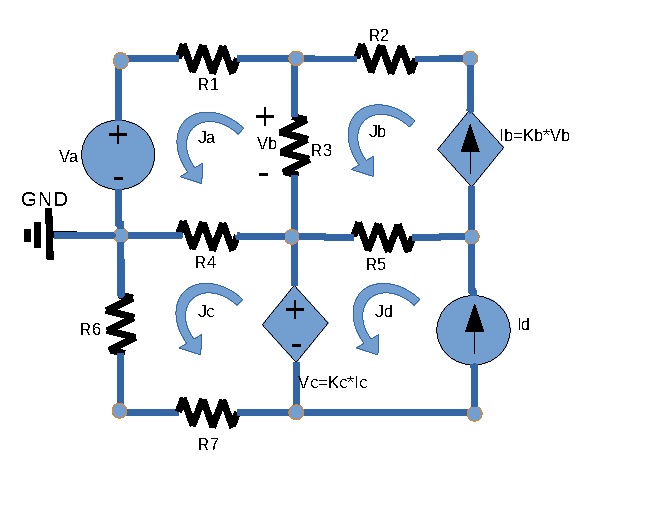
\includegraphics[width=0.55\linewidth]{t1_circuit_MM.pdf}
\caption{Circuit with mesh currents (Mesh Method).}
\label{fig:t1_circuit_MM}
\end{figure}


\par
According to this method, the algebraic sum of voltages around a loop equals zero or, in other way, the sum of voltage rises equals the sum of voltage drops around a loop. Applying this method the only unknown variables are the currents that circulate on each mesh. So, for mesh A:
\begin{equation}
  J_a\times R_1 + V_a + R_4\times (J_a - J_c) + R_3\times (J_a - J_b) = 0
  \label{eq:kvl}
\end{equation}

Mesh B:
\begin {equation}
  J_b = I_b = K_b\times V_b = K_b\times R_3\times (J_b - J_a)
  \label {eq:kvl}
\end{equation}

Mesh C:
\begin {equation}
  J_c\times R_7 - K_c\times J_c + R_4\times (J_c - J_a) + R_6\times J_c = 0
  \label {eq:kvl}
\end{equation}

And mesh D:
\begin {equation}
  J_d = I_d
  \label {eq:kvl}
\end{equation}
 
 By computing this four equations in function of the four variables: Ja, Jb, Jc e Jd. The values presented in Table~\ref{tab:MM} were obtained. For this calculations it was used the mathematical tool, Octave.

\begin{table}[h]
  \centering
  \begin{tabular}{|l|r|}
    \hline    
    {\bf Name} & {\bf Value [A]} \\ \hline
    Ja & -0.00022595\\ \hline
Jb & -0.00023645\\ \hline
Jc &  0.00095088\\ \hline
Jd &  0.0010264\\ \hline

  \end{tabular}
  \caption{Theoretical values obtained using octave to solve equations of mesh method.}
  \label{tab:MM}
\end{table}

\newpage

\subsection{Node Method}

\begin{figure}[h] \centering
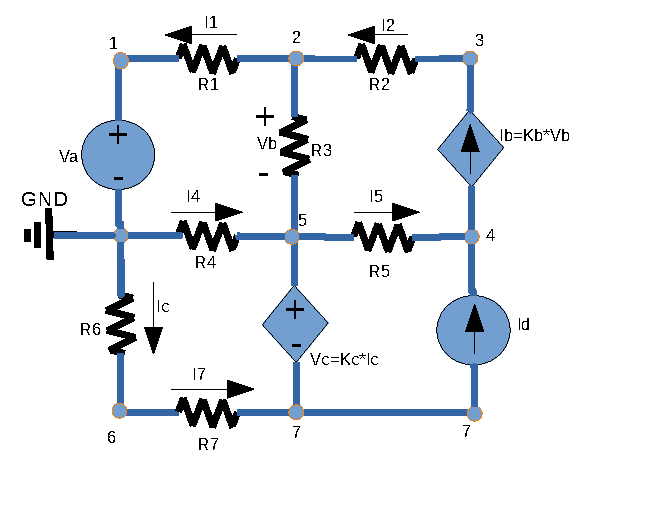
\includegraphics[width=0.6\linewidth]{t1_circuit_NM.pdf}
\caption{Circuit with currents and nodes identified (Node Method).}
\label{fig:t1_circuit_NM}
\end{figure}

In the same way, we can apply the node method, this method is based in the Kirchhoff's Current Law (KCL) and in the Ohm's Law, to analyse circuits. According to this method, KCL is applied in nodes that aren't connected to voltage sources and the currents flowing into a node must add up to zero, which means that the algebraic sum of currents that enters into a node equals to the algebraic sum of currents that exits that node. In nodes related by voltage sources, additional equations are applied. 
So, applying KCL for node 2, we have:
\begin {equation}
  (V_3 - V_2)\times G_2 = (V_2 - V_1)\times G_1 + (V_2 - V_5)\times G_3
  \label {eq:kvl}
\end{equation}

Node 3:
\begin{equation}
(V_3- V_2)\times G_2 = K_b\times (V_2 - V_5)
  \label {eq:kvl}
\end{equation}

Node 4:
\begin {equation}
I_d + (V_5 - V_4)\times G_5 = K_b\times (V_2 - V_5)
  \label {eq:kvl}
\end{equation}

And node 6:
\begin {equation}
(-V_5)\times G_6 = (V_6 - V_7)\times G_7
  \label {eq:kvl}
\end{equation}

The additional equations are:

\begin {equation}
V_1= V_a
  \label {eq:kvl}
\end{equation}

\begin {equation}
V_5 - V_1 = K_c\times (-V_6)\times G_6
  \label {eq:kvl}
\end{equation}

\begin {equation}
(V_6 - V_7)\times G_7 + (-V_5)\times G_4 + (V_2 - V_5)\times G_3 = (V_5 - V_4)\times G_5 + I_D
  \label {eq:kvl}
\end{equation}

The equations (9) and (10) are obtained using the voltage drop between the two voltage sources. The last equation was derived using a super-node that contains the dependent voltage source. Applying the node law, the sum of currents that enter the dependent voltage source is equal to the sum of currents that leaves it. 

\begin{table}[h]
  \centering
  \begin{tabular}{|l|r|}
    \hline    
    {\bf Name} & {\bf Value [A or V]} \\ \hline
    V0 & 0\\ \hline
V1 &  5.0102\\ \hline
V2 &  4.7774\\ \hline
V3 &  4.2972\\ \hline
V4 &  8.6049\\ \hline
V5 &  4.8099\\ \hline
V6 & -1.9313\\ \hline
V7 & -2.9274\\ \hline

  \end{tabular}
  \caption{Theoretical values obtained using octave to solve equations of Node Method.}
  \label{tab:NM}
\end{table}





